\chapter{Neutrino mass generation}
\label{sec:neutrino_mass}

The evidence for three neutrino flavour oscillation is well established~\cite{Fukuda:1998mi,Aharmim:2005gt} %
and can be accounted for only if neutrino mass splittings are non zero~\cite{nufit}.
This implies that neutrinos are massive and mix, forcing to consider extensions %
of the Standard Model (SM) to explain their origin. 
A simple means of doing so is to introduce the right-handed counterpart of SM neutrinos, which are %
singlet with respect to all SM gauge symmetries.
The Lagrangian includes a Yukawa coupling between these sterile states, the Higgs boson and the leptonic doublet, %
which generates Dirac mass-terms below the scale of Electroweak Symmetry Breaking (EWSB), 
and Majorana mass terms for the new singlet states.
On diagonalisation of the resulting neutrino mass matrix, the heavy neutrino states, %
commonly known as nearly-sterile neutrinos or Heavy Neutral Leptons (HNLs) in experimental contexts, %
remain mainly in the sterile neutrino direction and have sub-weak interactions suppressed by %
elements of the extended Pontecorvo-Maki-Nakagawa-Sakata (PMNS) mixing matrix. 

These states have been connected to a vast range of phenomenological behaviours and %
even to cosmological implications (for a recent review on sterile neutrinos, see \eg \refref{Abazajian:2012ys}).
For instance, nearly-sterile neutrinos in the keV region are viable warm Dark Matter candidates (see \eg \refref{Asaka:2005an}), %
whereas heavier HNLs could play a role in leptogenesis~\cite{Fukugita:1986hr, Covi:1996wh, Pilaftsis:1997jf, Buchmuller:1997yu, %
Pilaftsis:2003gt, Davidson:2008bu, Akhmedov:1998qx, Asaka:2005pn, Hernandez:2015wna, Hernandez:2016kel, %
Hambye:2016sby, Hambye:2017elz, Drewes:2017zyw}.
So far, some possible hints in favour of heavy neutrinos have emerged in neutrino appearance oscillation experiments, %
specifically LSND~\cite{Aguilar:2001ty} and MiniBooNE~\cite{Aguilar-Arevalo:2012fmn, Aguilar-Arevalo:2013pmq, Aguilar-Arevalo:2018gpe} %
but are disfavoured by disappearance experiments~\cite{TheIceCube:2016oqi, Adamson:2017uda, Aartsen:2017bap}, %
unless non-standard effects are present~\cite{Liao:2016reh, Liao:2018mbg, Esmaili:2018qzu, Denton:2018dqq}. Further hints 
in the same mass range have been reported for mixing with electron neutrinos in the so-called reactor anomaly~\cite{Mueller:2011nm, Mention:2011rk, Huber:2011wv, Ko:2016owz, Alekseev:2018efk} and in the less statistically significant Gallium one~\cite{Abdurashitov:2005tb, Laveder:2007zz, Giunti:2006bj}.
Explanations of the MiniBooNE low energy excess invoking GeV-scale HNLs with non-standard interactions~\cite{Gninenko:2009ks, Gninenko:2010pr, %
	Masip:2012ke, Bertuzzo:2018itn, Ballett:2018ynz}, %
have also been put forward. In these models, heavy neutral fermions are produced by neutrino up-scattering in the detector and subsequently decaying into photons or electrons, which mimic an electron neutrino interaction.
The interpretation of the current experimental results is still largely debated in the scientific community.
Searches both for electron-like signatures in MicroBooNE, the SBN programme at Fermilab~\cite{Antonello:2015lea}, %
and in short baseline reactor neutrino experiments, such as DANNS~\cite{Alekseev:2018efk}, NEOS~\cite{Ko:2016owz}, %
PROSPECT~\cite{Ashenfelter:2018iov}, STEREO~\cite{Almazan:2018wln}, NEUTRINO-4~\cite{Serebrov:2018vdw}, %
will shed further light on these possibilities.

Apart from these controversial hints, no positive evidence of heavy neutrinos has been found to date in laboratory searches.
A thorough review of the current constraints can be found in~\refrefs{Atre:2009rg, Drewes:2015iva}. 
%
%
%
%and studies of
%$0\nu\beta\beta$~\cite{Benes:2005hn} 
%
Bounds critically depend on the HNL masses and the flavour with which they mix.
Searches for kinks in Curie plots of $\beta$-decay
spectra~\cite{Galeazzi:2001py, Hiddemann:1995ce, Holzschuh:1999vy,
	Holzschuh:2000nj, Deutsch:1990ut} have placed bounds on the electronic
mixing for HNL masses between the keV and MeV scales.  
%
For masses from a few MeV to a few hundreds MeV, searches for monochromatic peaks in the lepton spectrum of decaying pions %
and kaons place important bounds on the muonic and electronic mixing angles~\cite{Artamonov:2014urb, Britton:1992pg, Britton:1992xv, Aguilar-Arevalo:2017vlf, Aguilar-Arevalo:2019owf}.
Neutrinoless double beta decay indirectly constrains Majorana HNLs from the eV to the TeV scale %
and lepton number violating meson and tau decays can be used to set limits on the mixing angle %
in narrow ranges of HNLs masses~\cite{Atre:2009rg}. 
%
%
The tightest constraints come from searches for the direct production and subsequent decays of heavy neutrinos %
in \emph{beam dump} experiments and at colliders.
%
The strongest limits were set by the PS191 experiment~\cite{Bernardi:1985ny, Bernardi:1987ek}, %
a beam dump experiment which ran at CERN in 1984.
Its most stringent upper bounds on the novel mixing angles are \mbox{$|U_{e4}|^2, |U_{\mu4}|^2 \leq \np{e-8} \text{\,--\,} \np{e-9}$} %
for neutrino masses between the pion and the kaon mass.
Other bounds of this type can be found in~\refrefs{Abreu:1996pa, Adriani:1992pq, Vilain:1994vg, Vaitaitis:1999wq, Badier:1985wg, CooperSarkar:1985nh, Gallas:1994xp}
as well as collider ones, from LHCb~\cite{Aaij:2014aba}, ATLAS~\cite{Aaboud:2018spl}, CMS~\cite{Sirunyan:2018mtv, Sirunyan:2018xiv}, BELLE~\cite{Liventsev:2013zz} %
(see also \refref{Harrison:2015bja}).

% Similarly, peak searches in leptonic decays
%at rest of pions and kaons have proved to be a very powerful probe of the
%mixing of heavy neutrinos with both $\nu_e$ and $\nu_\mu$.  If a heavy
%neutrino is produced in such decays, the lepton spectrum would show a
%monochromatic line at % \begin{equation} % E_\ell = \frac{M_0^2 + m_\ell^2 -
%m_N^2}{2 M_0} % \end{equation} % where $M_0$ is the decaying meson mass and
%$m_\ell$ the associated lepton.  Different experiments
%{E949~\cite{Artamonov:2014urb}, PIENU~\cite{PIENU:2011aa},
%TRIUMF~\cite{Britton:1992pg}~\cite{Britton:1992xv}} studied $\pi$ and $K$
%decays placing robust bounds.  % Searches for kinks in Curie plots of
%$\beta$-decay spectra~\cite{Galeazzi:2001py, Hiddemann:1995ce,
%Holzschuh:1999vy, Holzschuh:2000nj, Deutsch:1990ut} and studies of
%$0\nu\beta\beta$~\cite{Benes:2005hn} have placed bounds on the electronic
%mixing.  % A thorough review of the current constraints is found
%in~\cite{Atre:2009rg, Drewes:2015iva}.
%

It is exciting to note that current and upcoming neutrino oscillation
experiments will be able to perform beam dump style measurements \cite{Kusenko:2004qc, Asaka:2012bb, Abe:2019kgx}. 
%
A crucial difference between oscillation detectors and dedicated beam dump searches of the past is that %
the former tries to maximise its Standard Model neutrino scattering rate, while the latter goes to lengths %
to suppress it in order to reduce backgrounds.
%
However, for some of the current and future accelerator neutrino experiments, %
such as the Short Baseline Neutrino (SBN) program~\cite{Antonello:2015lea}, %
the strong particle reconstruction capabilities of Liquid Argon detectors and distinctive kinematics %
of neutrino decays have been shown to allow competitive bounds on heavy neutrinos %
to be made despite naively large backgrounds \cite{Ballett:2016opr}. 
%
Long baseline oscillation experiments, such as the upcoming Deep Underground Neutrino Experiment (DUNE)~\cite{Abi:2018dnh}, %
will see a greatly diluted flux of nearly-sterile neutrinos at their far detectors and consequently poor sensitivity.
However, the DUNE Near Detector (DUNE ND), placed \np{574}\,m from the target, has a great potential %
for searches for new physics~\cite{Adams:2013qkq}.
Even if the final design of the ND has not been confirmed as yet, the options being considered combine a large active volume, %
in close proximity to a very intense neutrino beam and cutting-edge event reconstruction capabilities.
These will allow DUNE ND to undertake valuable searches for BSM physics in a entirely complementary way %
to the central oscillation physics programme. 

In this article, we present a detailed analysis of the sensitivity of DUNE ND to HNL in beam dump style searches.
Differently from previous sensitivity studies \cite{Krasnov:2019kdc, Adams:2013qkq},  %
we ground our discussion in theoretically consistent models, in which sterile neutrinos are associated with neutrino %
mass generation via a low-scale seesaw mechanism. %, such as inverse seesaw (ISS) mechanisms.
We note that the range of masses and mixing angles testable at DUNE~ND is of interest for the generation of %
the baryon asymmetry in the context of the ASR mechanism~\cite{Akhmedov:1998qx, Asaka:2005pn, Hernandez:2015wna, Hernandez:2016kel, Drewes:2017zyw}.
We consider both Majorana and pseudo-Dirac states and calculate their decay and production rates, 
with careful consideration given to helicity arguments.
These formulae are then used to estimate the sensitivity of the experiment, %
taking into account the beam and detector performance capabilities thanks to simulations of both event and background signals.
We stress that DUNE will be able to extend the current limits on new fermionic singlets, %
including those with masses above 500\,MeV, probing models of theoretical significance for the generation of neutrino mass.
We show that bounds can be put also on the mixing with tau neutrinos, thanks to the high energy~beam.
%Ultimately, we show that DUNE will mostly (but not exclusively) be sensitive to pseudo-Dirac states.
%and this can have consequence for the signal and analysis strategies adopted by the collaboration.
%Also by considering the relationship between low-scale steriles and neutrino masses, %
%our predictions from DUNE can be correlated with constraints from other experiments such as searches for LNV and NSIs/non-unitarity. 
%

The article is organised as follows.
In \refsec{sec:model} we discuss neutrino mass generation and its consequences for heavy neutrinos in the mass range of interest.
%%%% SWAP %%%%
%%original%%
%In \refsec{sec:production} and \refsec{sec:decay}, we present the sterile neutrino production and decay rates accounting for both
%%new vers%%
In \refsec{sec:decay} and \refsec{sec:production}, we present the nearly-sterile neutrino decay and production rates accounting for both %
Majorana/(pseudo-)Dirac states and fully incorporating helicity effects and distributional information about the final-state observables. 
In \refsec{sec:experiment}, we turn to DUNE~ND, describing our assumptions about the experimental apparatus, %
our neutrino flux modelling, including a $\nu_\tau/\cj{\nu}_\tau$ simulation, %
the expected signal and the impact of backgrounds.
%
In \refsec{sec:results}, we quantify the sensitivity of DUNE ND to decays of heavy neutrino and, %
in \refsec{sec:combined}, its ability to constrain the parameter space of low-scale seesaw models.
Our concluding remarks are made in \refsec{sec:conclusions}.

\section{Heavy neutrinos in seesaw models}
\label{sec:model}

The lightness of the observed neutrino masses can be explained in a range of different scenarios. %
New SM-gauge singlet fermions are a feature common to many of them. 
The~most general Lagrangian  including a set of right-chiral gauge singlets 
$\{{\cal{N}}_i\}$ is given by 
%
\begin{equation}
	\label{eq:model}
	\mathcal{L}_{\text{SM}+\mathcal{N}} = \mathcal{L}_\text{SM} + i\, \cj{\mathcal{N}}_i \sh{\pd} \mathcal{N}_i + Y_{\alpha i} \cj{L}_\alpha \widetilde{H} \mathcal{N}_i + \frac{1}{2} (M_R)_{ij} \cj{\mathcal{N}^c}_i \mathcal{N}_j + \text{h.c.}\ ,
	%\mathcal{L}_{\text{SM}+N} = \mathcal{L}_\text{SM} + i \cj{N}_i \sh{\pd} N_i + Y_{\alpha i} \cj{L}_\alpha \tilde{H} N_i %
	%+ \frac{1}{2} (M_R)_{ij} \cj{N^c}_i N_j + \text{h.c.}\ ,
\end{equation}
%
with $\mathcal{L}_\text{SM}$ denoting the SM Lagrangian and the other symbols taking their conventional meaning.
Without loss of generality, $M_R$ can be chosen to be diagonal.
After electroweak symmetry breaking, a Dirac mass emerges for which we will use the notation $m_D \equiv v Y/\sqrt{2}$.
%
This term appears, for instance, in the famous Type I seesaw mechanism~\cite{Minkowski:1977sc,Mohapatra:1979ia,GellMann:1980vs,Yanagida:1979as}. %
Majorana masses for the light neutrinos arise and are given by
%
\begin{equation}
	\label{eq:typeI}
	m_\nu = -m_D M_R^{-1} m_D^T + \mathcal{O}\qty(\qty[m_D M_R^{-1}]^2)\ .
\end{equation}
%
The heavy neutrino masses are approximately given by the diagonal entries of $M_R$ and its corresponding eigenstates, %
the heavy nearly-sterile neutrinos $N_i$, have suppressed mixing with active neutrinos and are mainly composed %
by sterile fields.
Neglecting the matrix nature of these expressions for now, if $m_D$ takes values around the electroweak scale, %
acceptable neutrino masses are produced when $M_R$ has values around the GUT scale, %
suggestively connecting it to a high-scale breaking of $U(1)_{B-L}$~\cite{Minkowski:1977sc}.
Low-scale solutions are also possible by taking the Yukawa couplings to be similar %
or smaller than the other SM lepton Yukawa couplings, \eg if $m_D$ takes values in the keV range, %
new nearly-sterile states would exist with masses around a GeV.
%
Although the mass scale for the heavy neutrino can span many orders of magnitude, %
the resulting mixing is constrained by the contribution given to light neutrino masses
%
\begin{equation}
	\label{eq:TypeI_mixing_bound}
	\qty|U_{\alpha N}|^2 \lesssim \frac{m_\nu}{m_N} \lesssim  \np{e-10}\ \frac{1\,\mathrm{GeV}}{m_N}\ ,
	%
\end{equation}
%
where we have taken $m_\nu\lesssim 0.1$\,eV.
These suppressed mixing angles make experimental searches for heavy neutrinos in this range particularly challenging, %
and beyond the capabilities of most experiments to-date.

In recent years a lot of interest has focused on more complex models with multiple new fermion states, %
\eg the Inverse Seesaw~(ISS)~\cite{Mohapatra:1986bd, GonzalezGarcia:1988rw}, extended seesaw~\cite{Barr:2003nn} %
and linear seesaw models~\cite{Malinsky:2005bi,Kang:2006sn}.
%
In these cases the bound in Eq.~(\ref{eq:TypeI_mixing_bound}) can be avoided because of the cancellation between %
the contributions to neutrino masses by a different sterile neutrino.
For~definiteness, we will focus on the ISS model.
In this case, a quasi-preserved lepton number guarantees the specific texture of $M_R$ and $m_D$ %
and its small breaking is natural in the 't Hooft sense~\cite{tHooft:1980xss}.
%We will refer to such models as ``symmetry-protected''.

The physical spectrum of heavy neutrinos can be best understood in the Lepton Number Conserving (LNC) limit.
We use ISS\,$(a,b)$ to denote the model with $a$ $(b)$, $a,b\neq 0$, new gauge singlets of lepton number $+1$ $(-1)$.
Following \refeq{eq:model} and \refeq{eq:typeI}, the most general mass matrices are then given by 
%
\[
	m_D = \qty( \begin{matrix} m, 0\end{matrix}) \qquad \text{and}\qquad M_R = %
	\qty(\begin{matrix} 0 & M^\text{T} \\ M & 0 \end{matrix})\ ,
\]
%
where we introduce the $3\times a$ complex matrix $m$ and the $b\times a$ complex matrix $M$.
%
The spectrum of physical states in the LNC limit for ISS\,$(a,b)$ is given by
%
\[	
	%
	\text{min}\{3+b,a\}~\text{Dirac pairs}\qquad\text{and}\qquad
	|3 + b-a|~\text{massless Weyl states}.  
	%
\] 
%
The masses of the Dirac pairs are the non-zero singular values of the rectangular $a \times (3+b)$ matrix $(m^\text{T}, M^\text{T})$.
Note that for $a\neq b$, in addition to a set of Dirac pairs of arbitrary masses, extra massless sterile states %
degenerate with the light neutrinos are present.
Mixing involving these degenerate states is not defined in the LNC limit, as any unitary map in the degenerate subspace is permissible.
On the contrary, the introduction of a small Lepton Number Violating (LNV) parameter %
perturbs the LNC spectrum as well as the mixing.
In general there are only two possible origins for a low-scale heavy neutrino: 
%
 \begin{itemize}
			%
		\item A massless Weyl fermion in the LNC limit which is given non-zero mass proportional to the perturbation.
			As the mixing between massless states is not defined in the LNC limit, the perturbation controls %
			the induced mixing between the nearly-sterile state and the active ones.
			We will refer to this state as a Majorana neutrino.
			%
		\item A massive Dirac pair at the low scale in the LNC limit, becoming a pseudo-Dirac pair after the perturbation, %
			which regulates the mass splitting of the pair.
			In the LNC limit, the mixing angles between Dirac pair and light neutrinos can be arbitrarily large,
			and this property remains after the perturbation.
			%
	\end{itemize}
	%
	The first case only arises in models with an imbalanced number of new fields, %
	\ie ISS\,$(a,b)$ such that $a\neq b$, while the second option can occur in any ISS model. 

In this paper, we are interested in heavy states with masses in the MeV--GeV range.%
\footnote{This is motivated by the kinematic limits on production from meson decays discussed in more detail in \refsec{sec:production}.} %
Our discussion above suggests that both Majorana states and (pseudo-)Dirac states should be considered, %
covering all possible phenomenological aspects.
In what follows, we will compute the production and decay rates for Majorana states %
and Dirac states and study their discovery potential at DUNE ND.
We disregard lepton number violating effects and therefore the distinction between pseudo-Dirac and Dirac states will not be relevant.

Feynman rules for Majorana states derived from \refeq{eq:model} can be found in~\cite{Atre:2009rg},
or constructed using the techniques of \refref{Denner:1992me}. 
For an explicit comparison between Dirac versus Majorana Feynman rules for heavy neutrinos, see~\refref{Abada:2016plb}.



\section{Heavy neutrino decay}
\label{sec:decay}

In this section we compute the heavy neutrino decay rates and polarised %
distributions necessary for the simulation of beam dump searches.
We compute rates for both Majorana and (pseudo-)Dirac states, allowing us to consistently %
explore the parameter space of low-scale seesaw models.
%
%If the new neutrinos are massive enough, their mass-splittings with the light
%neutrinos could be larger than the wave packet energy-uncertainty associated
%with the production mechanism and they no longer
%oscillate~(see \eg\ \refref{Akhmedov:2009rb}). Instead, the neutrinos are stable enough to
%propagate to a short-baseline detector and decay into visible SM particles.
%%
%In this section we discuss the decay rates of Majorana and (pseudo-)Dirac 
%sterile neutrinos for their most promising signatures, taking particular care
%over the polarization of the beam discussed in the previous section.

This analysis can be simplified by noting the following equivalences.
A Majorana neutrino $N$ decaying via a charged current process has the same differential %
decay rate as the Dirac neutrino $N_D$ with the appropriate lepton number, 
\[
	\dd{\Gamma}(N\to \ell_\alpha^- X^+) = \dd{\Gamma}(N_D\to \ell_\alpha^- X^+) \quad\text{and}\quad
	\dd{\Gamma}(N\to \ell_\alpha^+ X^-) = \dd{\Gamma}(\cj{N}_D\to \ell_\alpha^+ X^-)\ ,
\]
%
where we assume identical mass and mixing angles for both Dirac and Majorana neutrinos. 
%
This equivalence can be seen directly from the Feynman rules for Dirac and Majorana fermions~\cite{Denner:1992me} %
(see also \refref{Abada:2016plb}), but also explicitly in our formulae below.
%
In a neutral current (NC) decay, however, the two contractions of the NC operator lead to another contribution,  
%
\begin{equation*}
	%\label{eq:gamma_NC_sum}
	\dd{\Gamma}(N \to \nu X') = \dd{\Gamma}(N_D\to \nu X') + \dd{\Gamma}(\cj{N}_D\to\cj{\nu} X')\ .
\end{equation*}
%
These relations hold at the differential level if the kinematic variables are reinterpreted in the obvious way.
In this sense, we can view the Majorana process as the sum of Dirac particle and antiparticle decays.%
\footnote{In a general amplitude with Majorana states, there would also be an interference contribution between these two %
	sub-processes. However, in all cases of interest, interference diagrams are proportional to the %
	final-state light neutrino mass, which we take to be zero.} 
%
%If we consider the total decay rates only, we can make a further
%simplification if $Y$ is its own CP conjugate, $Y=\overline{Y}$. As CP
%violation requires the interference of strong and weak phases \cite{}, at
%tree-level these processes are identical $\Gamma(\overline{\nu}\to
%\overline{\nu} Y) = \Gamma(\overline{\nu}\to \overline{\nu} \overline{Y}) =
%\Gamma(\nu \to \nu Y)$.
%
Considering the total decay rates only, we find that the Majorana decay is larger by a factor of 2 compared to the Dirac case,
\[
	\Gamma(N\to \nu X' ) = 2\Gamma(N_D \to \nu X')\ .
\]
%
Note that this is true only for the total decay rates with massless final-state neutrinos.

\begin{table}
	\small
	\centering
	\begin{tabular}{lrlrlr}
		\toprule                                    
		Channel			& Threshold		    &      Channel			& Threshold		&   Channel			& Threshold		\\
		\cmidrule(lr){1-2} \cmidrule(lr){3-4} \cmidrule(lr){5-6}                                   
		$\nu \nu \nu$		& \np{e-9}\,MeV	&  $e^\mp K^\pm$	    & \np{494}\,MeV		&   $\nu \eta'$		        & \np{958}\,MeV		\\
		$\nu e^+ e^-$		& \np{1.02}\,MeV&  $\nu \eta$	        & \np{548}\,MeV		&   $\mu^\mp K^{*\pm}$		& \np{997}\,MeV		\\
		$\nu e^\pm \mu^\mp$	& \np{105}\,MeV	&  $\mu^\mp K^\pm$      & \np{559}\,MeV		&   $\nu \phi$		        & \np{1019}\,MeV		\\
		$\nu \pi^0$ 		& \np{135}\,MeV	&  $\nu \rho^0$	        & \np{776}\,MeV		&   $\nu e^\pm \tau^\mp$	& \np{1776}\,MeV		\\
		$e^\mp \pi^\pm$		& \np{140}\,MeV	&  $e^\mp \rho^\pm$	    & \np{776}\,MeV		&   $e^\mp D^\pm$           & \np{1870}\,MeV		\\
		$\nu \mu^+ \mu^-$	& \np{210}\,MeV	&  $\nu \omega$	        & \np{783}\,MeV		&   $\nu \mu^\pm \tau^\mp$	& \np{1880}\,MeV		\\
		$\mu^\mp \pi^\pm$	& \np{245}\,MeV	&  $\mu^\mp \rho^\pm$	& \np{882}\,MeV		&   $\tau^\mp \pi^\pm$		& \np{1870}\,MeV		\\
		&               &  $e^\mp K^{*\pm}$	    & \np{892}\,MeV		&                           &                       \\
		\bottomrule
	\end{tabular}
	\footnotesize
	\caption{All the available channels for a HNL with a mass below the $D_s^\pm$ mass are listed above, %
		sorted by threshold mass.
		The active neutrino is considered massless, when compared to the masses of the other particles.}
	\label{tab:decays}
\end{table}

It is instructive to reconsider this result in the light of the \emph{practical Dirac--Majorana confusion theorem}~\cite{Kayser:1981nw, %
	Kayser:1982br}.
In \refref{Kayser:1981nw}, the decomposition into particle and antiparticle processes was performed for %
Majorana neutrino--electron scattering via neutral current, leading to a factor of two enhancement in the total rate.
However, this enhancement was shown to be absent in practice due to the polarisation of the incoming neutrino, %
which suppresses the $\Delta L = 2$ contributions by factors of the neutrino mass. 
%
In the present case of nearly-sterile decay, where mass effects are large and essential to the calculation, %
there is no analogous effect: Dirac and Majorana neutrinos will have distinct total decay rates regardless of their polarisation. 
%
%In fact, we note that the helicity state of a massive fermion can never affect
%its total decay rate.%
%\footnote{This can be argued from the arbitrariness of the polarisation direction in the particle's rest frame, %
%or from the frame dependence of helicity for massive particles.}
%
Therefore, the total decay rates of heavy neutrinos into observable final states could in principle allow us to determine %
the Majorana/Dirac nature of the initial state.
This is not a trivial effect: a pure Majorana state decays with equal probability into $e^-\pi^+$ as $e^+ \pi^-$, %
one of its dominant and most experimentally distinctive branching decay modes, while a Dirac heavy neutrino %
will only decay into $e^-\pi^+$.
%
Assuming charge-identification is possible in the detector, distinguishing between the two total decay rates %
should be possible with modest statistics. %
%\footnote{Even if charged-ID is not available, some distributional distinctions can be made in principle, as we discuss later.}
In a charge-blind search or for an NC channel, the total decay rate of Majorana neutrinos would appear to be twice as large as that of Dirac neutrinos.
However, being the mixing usually an unknown quantity, the difference between Majorana and Dirac nature cannot be deduced as easily.

There is also a more subtle impact of the nature of the decaying neutrino.
%
Even though the total decay rate is not affected by the helicity of the initial neutrino, %
the helicity does affect the distributions of final state particles, which will in turn influence the observability of %
the signatures of neutrino decay. 
%
It is important that these polarisation effects are correctly implemented when studying the distributions of %
final state observables and subsequently when developing an analysis to tackle backgrounds. 

In the remainder of this section, we present results for the polarised heavy neutrino decay rates %
and distributions for Majorana and (pseudo-)Dirac neutrinos.
The decay modes considered are listed in~\reftab{tab:decays} and the respective branching ratios as functions of %
the neutrino mass are shown in~\reffig{fig:branch}.
%
The differential widths have been computed using the massive spinor helicity formalism %
(see \eg \refrefs{Dittmaier:1998nn, Diaz-Cruz:2016ahc}), and checked numerically using %
FeynCalc~\cite{Shtabovenko:2016sxi,Mertig:1990an}.

\begin{figure}
	\centering
	%\resizebox{\textwidth}{!}{% GNUPLOT: LaTeX picture with Postscript
\begingroup
  \makeatletter
  \providecommand\color[2][]{%
    \GenericError{(gnuplot) \space\space\space\@spaces}{%
      Package color not loaded in conjunction with
      terminal option `colourtext'%
    }{See the gnuplot documentation for explanation.%
    }{Either use 'blacktext' in gnuplot or load the package
      color.sty in LaTeX.}%
    \renewcommand\color[2][]{}%
  }%
  \providecommand\includegraphics[2][]{%
    \GenericError{(gnuplot) \space\space\space\@spaces}{%
      Package graphicx or graphics not loaded%
    }{See the gnuplot documentation for explanation.%
    }{The gnuplot epslatex terminal needs graphicx.sty or graphics.sty.}%
    \renewcommand\includegraphics[2][]{}%
  }%
  \providecommand\rotatebox[2]{#2}%
  \@ifundefined{ifGPcolor}{%
    \newif\ifGPcolor
    \GPcolortrue
  }{}%
  \@ifundefined{ifGPblacktext}{%
    \newif\ifGPblacktext
    \GPblacktexttrue
  }{}%
  % define a \g@addto@macro without @ in the name:
  \let\gplgaddtomacro\g@addto@macro
  % define empty templates for all commands taking text:
  \gdef\gplbacktext{}%
  \gdef\gplfronttext{}%
  \makeatother
  \ifGPblacktext
    % no textcolor at all
    \def\colorrgb#1{}%
    \def\colorgray#1{}%
  \else
    % gray or color?
    \ifGPcolor
      \def\colorrgb#1{\color[rgb]{#1}}%
      \def\colorgray#1{\color[gray]{#1}}%
      \expandafter\def\csname LTw\endcsname{\color{white}}%
      \expandafter\def\csname LTb\endcsname{\color{black}}%
      \expandafter\def\csname LTa\endcsname{\color{black}}%
      \expandafter\def\csname LT0\endcsname{\color[rgb]{1,0,0}}%
      \expandafter\def\csname LT1\endcsname{\color[rgb]{0,1,0}}%
      \expandafter\def\csname LT2\endcsname{\color[rgb]{0,0,1}}%
      \expandafter\def\csname LT3\endcsname{\color[rgb]{1,0,1}}%
      \expandafter\def\csname LT4\endcsname{\color[rgb]{0,1,1}}%
      \expandafter\def\csname LT5\endcsname{\color[rgb]{1,1,0}}%
      \expandafter\def\csname LT6\endcsname{\color[rgb]{0,0,0}}%
      \expandafter\def\csname LT7\endcsname{\color[rgb]{1,0.3,0}}%
      \expandafter\def\csname LT8\endcsname{\color[rgb]{0.5,0.5,0.5}}%
    \else
      % gray
      \def\colorrgb#1{\color{black}}%
      \def\colorgray#1{\color[gray]{#1}}%
      \expandafter\def\csname LTw\endcsname{\color{white}}%
      \expandafter\def\csname LTb\endcsname{\color{black}}%
      \expandafter\def\csname LTa\endcsname{\color{black}}%
      \expandafter\def\csname LT0\endcsname{\color{black}}%
      \expandafter\def\csname LT1\endcsname{\color{black}}%
      \expandafter\def\csname LT2\endcsname{\color{black}}%
      \expandafter\def\csname LT3\endcsname{\color{black}}%
      \expandafter\def\csname LT4\endcsname{\color{black}}%
      \expandafter\def\csname LT5\endcsname{\color{black}}%
      \expandafter\def\csname LT6\endcsname{\color{black}}%
      \expandafter\def\csname LT7\endcsname{\color{black}}%
      \expandafter\def\csname LT8\endcsname{\color{black}}%
    \fi
  \fi
    \setlength{\unitlength}{0.0500bp}%
    \ifx\gptboxheight\undefined%
      \newlength{\gptboxheight}%
      \newlength{\gptboxwidth}%
      \newsavebox{\gptboxtext}%
    \fi%
    \setlength{\fboxrule}{0.5pt}%
    \setlength{\fboxsep}{1pt}%
\begin{picture}(14400.00,5040.00)%
    \gplgaddtomacro\gplbacktext{%
      \csname LTb\endcsname%%
      \put(444,440){\makebox(0,0)[r]{\strut{}\np{e-5}}}%
      \put(444,1360){\makebox(0,0)[r]{\strut{}\np{e-4}}}%
      \put(444,2280){\makebox(0,0)[r]{\strut{}\np{e-3}}}%
      \put(444,3199){\makebox(0,0)[r]{\strut{}\np{e-2}}}%
      \put(444,4119){\makebox(0,0)[r]{\strut{}\np{e-1}}}%
      \put(444,5039){\makebox(0,0)[r]{\strut{}\np{1}}}%
      \put(576,220){\makebox(0,0){\strut{}$0$}}%
      \put(2304,220){\makebox(0,0){\strut{}$0.5$}}%
      \put(4032,220){\makebox(0,0){\strut{}$1$}}%
      \put(5759,220){\makebox(0,0){\strut{}$1.5$}}%
    }%
    \gplgaddtomacro\gplfronttext{%
      \csname LTb\endcsname%%
      \put(-304,2739){\rotatebox{-270}{\makebox(0,0){\strut{}Branching ratio (\%)}}}%
      \put(4031,-110){\makebox(0,0){\strut{}Mass (GeV)}}%
      \csname LTb\endcsname%%
      \put(4836,2169){\makebox(0,0)[l]{\strut{}$e^\mp\pi^\pm$}}%
      \csname LTb\endcsname%%
      \put(4836,1905){\makebox(0,0)[l]{\strut{}$\mu^\mp\pi^\pm$}}%
      \csname LTb\endcsname%%
      \put(4836,1641){\makebox(0,0)[l]{\strut{}$e^\mp K^\pm$}}%
      \csname LTb\endcsname%%
      \put(4836,1377){\makebox(0,0)[l]{\strut{}$\mu^\mp K^\pm$}}%
      \csname LTb\endcsname%%
      \put(4836,1113){\makebox(0,0)[l]{\strut{}$e^\mp\rho^\pm$}}%
      \csname LTb\endcsname%%
      \put(4836,849){\makebox(0,0)[l]{\strut{}$\mu^\mp\rho^\pm$}}%
      \csname LTb\endcsname%%
      \put(5823,2169){\makebox(0,0)[l]{\strut{}$e^\mp K^{*\pm}$}}%
      \csname LTb\endcsname%%
      \put(5823,1905){\makebox(0,0)[l]{\strut{}$\mu^\mp K^{*\pm}$}}%
      \csname LTb\endcsname%%
      \put(5823,1641){\makebox(0,0)[l]{\strut{}$e^\mp D^\pm$}}%
      \csname LTb\endcsname%%
      \put(5823,1377){\makebox(0,0)[l]{\strut{}$\nu e^\mp\mu^\pm$}}%
      \csname LTb\endcsname%%
      \put(5823,1113){\makebox(0,0)[l]{\strut{}$\nu e^\mp\tau^\pm$}}%
      \csname LTb\endcsname%%
      \put(5823,849){\makebox(0,0)[l]{\strut{}$\tau^\mp\pi^\pm$}}%
    }%
    \gplgaddtomacro\gplbacktext{%
      \csname LTb\endcsname%%
      \put(7355,440){\makebox(0,0)[r]{\strut{}}}%
      \put(7355,1360){\makebox(0,0)[r]{\strut{}}}%
      \put(7355,2280){\makebox(0,0)[r]{\strut{}}}%
      \put(7355,3199){\makebox(0,0)[r]{\strut{}}}%
      \put(7355,4119){\makebox(0,0)[r]{\strut{}}}%
      \put(7355,5039){\makebox(0,0)[r]{\strut{}}}%
      \put(14399,220){\makebox(0,0){\strut{}$2$}}%
      \put(7487,220){\makebox(0,0){\strut{}$0$}}%
      \put(9215,220){\makebox(0,0){\strut{}$0.5$}}%
      \put(10943,220){\makebox(0,0){\strut{}$1$}}%
      \put(12671,220){\makebox(0,0){\strut{}$1.5$}}%
    }%
    \gplgaddtomacro\gplfronttext{%
      \csname LTb\endcsname%%
      \put(10943,-110){\makebox(0,0){\strut{}Mass (GeV)}}%
      \csname LTb\endcsname%%
      \put(12093,2424){\makebox(0,0)[l]{\strut{}$\nu\nu\nu$}}%
      \csname LTb\endcsname%%
      \put(12093,2160){\makebox(0,0)[l]{\strut{}$\nu e^+ e^-$}}%
      \csname LTb\endcsname%%
      \put(12093,1896){\makebox(0,0)[l]{\strut{}$\nu\mu^+ \mu^-$}}%
      \csname LTb\endcsname%%
      \put(12093,1632){\makebox(0,0)[l]{\strut{}$\nu\pi^0$}}%
      \csname LTb\endcsname%%
      \put(12093,1368){\makebox(0,0)[l]{\strut{}$\nu\rho^0$}}%
      \csname LTb\endcsname%%
      \put(13212,2424){\makebox(0,0)[l]{\strut{}$\nu\omega$}}%
      \csname LTb\endcsname%%
      \put(13212,2160){\makebox(0,0)[l]{\strut{}$\nu\eta$}}%
      \csname LTb\endcsname%%
      \put(13212,1896){\makebox(0,0)[l]{\strut{}$\nu\eta'$}}%
      \csname LTb\endcsname%%
      \put(13212,1632){\makebox(0,0)[l]{\strut{}$\nu\phi$}}%
    }%
    \gplbacktext
    \put(0,0){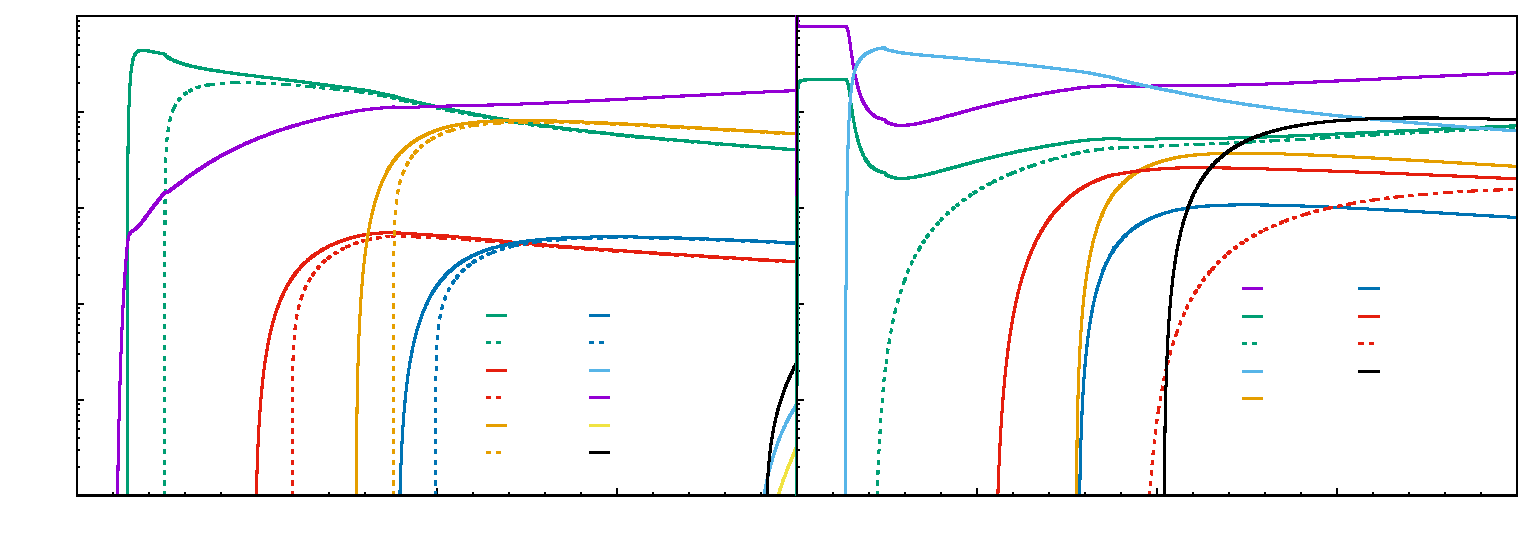
\includegraphics{pics/multiBranch}}%
    \gplfronttext
  \end{picture}%
\endgroup}
	\footnotesize
	\caption{The branching ratios for HNL decays, integrated over the angular variables, are shown above %
		as functions of the mass.
		They are grouped in CC-mediated decays (left) and NC-mediated decays (right), in the range from \np{0.01}\,MeV up to %
		the maximum mass limit for neutrino production, near 2\,GeV. 
		A scenario in which $|U_{e N}|^2=|U_{\mu N}|^2=|U_{\tau N}|^2$ is chosen here %
		for illustrative purposes.
		The branching ratios of Majorana neutrinos and Dirac neutrinos are mathematically identical and %
		therefore no distinction is stressed.
		%The semi-leptonic decays to $\pi$ mesons are the dominant ones, together with decays into pairs of charged leptons.
		The decay into three light neutrinos is fundamental for a correct computation %
		of the branching ratios, even though fully invisible from an experimental point of~view.}
	\label{fig:branch}
\end{figure}

\subsection{Polarised Majorana neutrino decay}

Although spin-averaged Majorana neutrino decay rates are well known in the literature~\cite{Atre:2009rg,Gorbunov:2007ak,Helo:2010cw} %
(see also Ref.~\cite{Bondarenko:2018ptm}), to the best of our knowledge the polarised rates are not.
These are necessary to correctly describe the distributions of observables in a beam dump experiment, %
and in this section we present formulae for these differential decay rates. 

\newpage
Note that we stay agnostic as to the final nature and flavours of outgoing %
neutrinos, and in all cases sum over any possible outgoing states to define a %
semi-inclusive decay rate into the visible particle(s) $X'$, \ie 
%
\[
	\Gamma(N\to \nu X') \equiv \sum_{i=1}^3 \Gamma(N\to\nu_i X')\ .
\]
%
The alternative, chosen by many other authors, is to treat light neutrinos as Dirac particles, %
and construct the full decay width using arguments of CP invariance, %
in practice amounting to adding some judicious factors of two~\cite{Atre:2009rg,Bondarenko:2018ptm}.
Following this approach, our summed decay rate for $N\to\nu X'$ can be seen as 
%
\[
	\Gamma(N\to \nu X') \equiv \sum_{\alpha=e}^\tau \qty[\Gamma(N\to\nu_\alpha X') + %
	\Gamma(N\to\overline{\nu}_\alpha X')]\ .
\]
%
The two approaches are identical mathematical procedures and can both be used to compute the differential decay rates; %
however, we avoid the latter as the light neutrinos in most seesaw models are Majorana fermions, and making a distinction %
between $\nu_\alpha$ and $\overline{\nu}_\alpha$ is physically misleading.%
\footnote{The approach could be seen as a short-hand for decay rates into polarised massless neutrinos, %
	but as we are particularly concerned with polarisation effects in the beam this only adds a further complication.}
We also find that the distribution of events, the role of helicity and the heavy neutrino nature are obscured by this approach.
%
In contrast, by summing over all outgoing states, our formulae are insensitive to the Majorana/Dirac nature of the light neutrinos, %
and are the physically relevant rates necessary for comparison with beam dump experiments, as outgoing neutrinos are not reconstructed.

\subsubsection{Pseudoscalar mesons}
\label{sec:pseudoscalar}

The semi-leptonic meson decays are some of the most important channels identified in previous studies~\cite{Atre:2009rg, %
	Ballett:2016opr} (see also \refref{Asaka:2012bb}) %
thanks to their large branching ratios and distinctive final state particles.
Both charged and neutral pseudo-scalar mesons are viable final state particles, namely $P^\pm$ and $P^0$, %
and the decay widths are given in the Centre of Mass (CM) frame by
%
\begin{align}
	\dv{\Gamma_\pm}{\Omega_{\ell_\alpha}} \qty(N \to \ell_\alpha^- P^+) &= %
	|U_{\alpha N}|^2|V_{q\, \cj{q}}|^2  \frac{G_\text{F}^2f_P^2 m_N^3}{16\pi} %
	\ I^\pm_1 \qty(\xi^2_\alpha, \xi^2_P; \theta_\alpha)\ ,\label{eq:M_decay_pseudo_plus}\\
	\dv{\Gamma_\pm}{\Omega_{\ell_\alpha}} \qty(N \to \ell_\alpha^+ P^-) &= %
	|U_{\alpha N}|^2|V_{q\, \cj{q}}|^2  \frac{G_\text{F}^2f_P^2m_N^3}{16\pi} %
	\ I^\mp_1 \qty(\xi^2_\alpha, \xi^2_P; \theta_\alpha)\ ,\label{eq:M_decay_pseudo_minus}\\
	\dv{\Gamma_\pm}{\Omega_P} \qty(N \to \nu P^0)\hphantom{{}^-} &= %
	\qty(\sum_{\alpha=e}^\tau| U_{\alpha N}|^2) \frac{G_\text{F}^2f_{P^0}^2m_N^3}{16\pi} %
	\ \frac{I_1 \qty(0, \xi^2_P)}{4\pi}\ ,\label{eq:M_decay_pseudo_0}
\end{align}
%
where $\Gamma_h$ is the decay rate for neutrinos of helicity $h$, %
$V_{q \cj{q}}$ is the appropriate CKM matrix element for the considered meson, $f_P$ is its decay constant %
and $\xi_i = m_i/m_N$ denotes the mass of the final state particle $i$ %
as a fraction of the initial state mass. 
The solid angle elements $\Omega_{\ell_\alpha}$ and $\Omega_P$ refer respectively to the charged lepton and %
pseudo-scalar meson angle with respect to the neutrino direction.
%
The kinematic function $I_1(x,y)$~\cite{Atre:2009rg} and its angular generalisation accounting for helicity, $I_1^\pm(x,y;\theta)$, %
are defined in \refapp{app:integrals}.
%
After integrating over the angular variables, we find that %
both the pseudo-scalar meson decay rates do not depend on helicity, as expected,
%
%	\begin{align*}
%		\Gamma_\pm \qty(N \to \ell_\alpha^- P^+) &= %
%		\frac{G_F^2}{16\pi} f_P^2\, |V_{q\, \cj{q}}|^2\, |U_{\alpha 4}|^2 m_N^3\,\lambda^\frac{1}{2}(1, \xi_\alpha, \xi_P) %
%		\qty[(1-\xi_\alpha)^2 - \xi_P(1+\xi_\alpha)]\ ,\\
%		\Gamma_\pm \qty(N \to \nu_\alpha P^0) &= 
%		\frac{G_F^2}{16\pi} f_P^2\, |U_{\alpha 4}|^2 m_N^3\, \qty(1-\xi_P^2)^2\ .
%	\end{align*}
%
\begin{align}
	\Gamma_\pm \qty(N \to \ell_\alpha^- P^+) &= \Gamma_\pm \qty(N \to \ell_\alpha^+ P^-) = %
	|V_{q\, \cj{q}}|^2 |U_{\alpha N}|^2 \frac{G_F^2f_P^2m_N^3}{16\pi}\ I_1\qty(\xi^2_\alpha, \xi^2_P)\ ,\\
	\Gamma_\pm \qty(N \to \nu P^0)\hphantom{{}^-} &= \left(\sum_{\alpha=e}^\tau|U_{\alpha N}|^2\right) %
	\frac{G_F^2f_P^2m_N^3}{16\pi}\ I_1\qty(0,\xi^2_P)\ .
\end{align}
%
These rates agree with those presented in \refrefs{Bondarenko:2018ptm,Gorbunov:2007ak} %
(correcting a factor of two discrepancy in the $\nu P^0$ rate of \refrefs{Atre:2009rg,Helo:2010cw}).

The decay into a neutral meson, in \refeq{eq:M_decay_pseudo_0}, is isotropic in the rest frame, while the charged-pion modes, %
\refeqs{eq:M_decay_pseudo_plus}{eq:M_decay_pseudo_minus}, inherit their angular dependence from $I^\pm(x, y; \theta_\alpha)$, %
on the lepton angle to the beam line in the heavy neutrino rest frame $\theta_\alpha$.
%
The isotropy of the neutral current decay $N\to\nu P^0$ is a manifestation of %
the Majorana nature of the particle, in agreement with the discussion of \refref{Balantekin:2018ukw}.
It is worth noting that, if final states are not charge-identified, a similar isotropy %
is obtained for the total rate of charged semi-leptonic decays, 
%
\begin{align}  
	%
	\dv{\Gamma_\pm}{\Omega_{\ell_\alpha}} \qty(N \to \ell_\alpha P) &\equiv
	\dv{\Gamma_\pm}{\Omega_{\ell_\alpha}} \qty(N \to \ell_\alpha^+ P^-) +
	\dv{\Gamma_\pm}{\Omega_{\ell_\alpha}} \qty(N \to \ell_\alpha^- P^+) \notag \\
	%
	&= |U_{\alpha N}|^2|V_{q\, \cj{q}}|^2  \frac{G_\text{F}^2f_P^2m_N^3}{16\pi}
	\ \frac{I_1 \qty(\xi^2_\alpha, \xi^2_P)}{2\pi}\ . 
	%
\end{align}
%

The formulae above apply for all pseudo-scalar mesons which are kinematically allowed.
For instance, below the $K^0$ mass, the heavy neutrino can decay only into pions, %
but above $\eta$ and $\eta'$ can be allowed in the final state.
%but for heavier masses 
%However, for steriles produced by $D_s$ meson decay, a charged kaon in the final state is also possible.
%For masses towards the upper limit of our range, decays into $\tau$ final states are also possible, %
%\eg $N \to \tau^\mp \pi^\pm$, but the smaller phase space makes them negligible for the present work.
%The same conclusion is true for the mode $e^\mp D^\pm$.
%	
% The neutral pion is the only neutral pseudoscalar meson below the $K^0$ mass.
%Above this limit, the channels with an $\eta$ or an $\eta'$ in the final state become allowed.
%The majority of neutral pseudoscalar mesons decay electromagnetically into two photons or multi-pion final states. 

\subsubsection{Vector mesons}

Although only for higher masses, HNL can also decay into vector mesons $V$, %
both via charged current, $N \to \ell^\mp V^\pm$, and neutral current, $N \to \nu V^0$.
We find the following polarised differential distributions in the heavy neutrino rest frame, 
%
\begin{align}
	\dv{\Gamma_\pm}{\Omega_{\ell_\alpha}} \qty(N \to \ell_\alpha^- V^+) &= %
	|U_{\alpha N}|^2 |V_{q\, \cj{q}}|^2 \frac{G_\text{F}^2f_V^2 m_N^3}{16\pi} %
	\ I^\pm_2\qty(\xi^2_\alpha, \xi^2_V; \theta_\alpha)\ ,\label{eq:M_decay_vector_plus}\\
	\dv{\Gamma_\pm}{\Omega_{\ell_\alpha}} \qty(N \to \ell_\alpha^+ V^-) &= %
	|U_{\alpha N}|^2  |V_{q\, \cj{q}}|^2\frac{G_\text{F}^2f_V^2m_N^3}{16\pi} %
	\ I^\mp_2 \qty(\xi^2_\alpha, \xi^2_V; \theta_\alpha)\ ,\label{eq:M_decay_vector_minus}\\
	\dv{\Gamma_\pm}{\Omega_V} \qty(N \to \nu V^0)\hphantom{{}^-} &= %
	\qty(\sum_{\alpha=e}^\tau| U_{\alpha N}|^2 ) %
	\frac{G_\text{F}^2f_{V}^2\kappa_V^2m_N^3}{16\pi}\ \frac{I_2 \qty(0, \xi^2_V)}{4\pi}\label{eq:M_decay_vector_0}\ ,
\end{align}
%
where $I_2(x,y)$ and $I_2^\pm(x,y;\theta)$ are defined in \refapp{app:integrals}.
%
We find the total decay widths given by
%
\begin{align}
	\Gamma\qty(N \to \ell_\alpha^- V^+) &=  \Gamma\qty(N \to \ell_\alpha^+ V^-) = %
	|U_{\alpha N}|^2 |V_{q\,\cj{q}}|^2 \frac{G_F^2 f_V^2m_N^3}{16\pi}\ I_2\qty(\xi^2_\alpha,\xi^2_V)\ ,\\
	\Gamma\qty(N \to \nu V^0)\hphantom{{}^-} &= \left(\sum_{\alpha = e}^\tau |U_{\alpha N}|^2\right) %
	\frac{G_F^2f_V^2\kappa_V^2  m_N^3}{16\pi}\ I_2\qty(0,\xi^2_V)\ ,
\end{align}
%
where the constants $\kappa_V$ are combinations of the Weinberg angle, depending on the flavour structure of $V^0$ (see below).
Our charged pseudo-vector decay rates agrees with \refrefs{Bondarenko:2018ptm, Atre:2009rg, Helo:2010cw, Gorbunov:2007ak} while %
our neutral pseudo-scalar calculation agrees with the corrected version presented in \refref{Bondarenko:2018ptm}.

As with the pseudo-scalar meson decay rates, the Majorana nature leads to an isotropic decay into a neutral vector meson.
An analogous effect holds for the charged vector meson decay if we assume that the charges of final state particles %
are not distinguished.
In this case, we find the physically relevant decay distribution in the particle rest frame to be given~by
%
\begin{align}
	%
	\dv{\Gamma_\pm}{\Omega_{\ell_\alpha}} \qty(N \to \ell_\alpha V) &\equiv \dv{\Gamma_\pm}{\Omega_{\ell_\alpha}} %
	\qty(N \to \ell_\alpha^- V^+) + \dv{\Gamma_\pm}{\Omega_{\ell_\alpha}} \qty(N \to \ell_\alpha^+ V^-)\ , \notag\\
	%
	&= |U_{\alpha N}|^2 \frac{G_\text{F}^2f_V^2}{16\pi} |V_{q\, \cj{q}}|^2\, m_N^3 %
	\ \frac{I_2 \qty(\xi^2_\alpha, \xi^2_V)}{2\pi}\ .
	%
\end{align}
%
There are no vector mesons lighter than the $K^0$, and these decays become relevant only for higher masses %
for which decays into $\rho^\pm$ and $K^{*\pm}$, and for the neutral mode into $\rho^0$, $\omega$, and $\phi$ would be relevant.
For these neutral particles, the $\kappa_V$ factors read
\[
	\kappa_\rho   = 1-\sin^2\theta_W \quad,\quad
	\kappa_\omega = \frac{4}{3} \sin^2\theta_W \quad,\quad
	\kappa_\phi   = \frac{4}{3} \sin^2\theta_W -1\ .
\]
%Vector mesons usually into a multi-state of pseudoscalar mesons, depending on the initial flavour content,
%sometimes accompanied by photon emission making their reconstruction challenging from an experimental point of view.

\subsubsection{Charged lepton pairs}

%The differential decay rates for these modes are more complicated to write
%down, but we give compact formulae for these channels in
%App.~\ref{app:threebody_dist}. 
%
We assign the momenta to the particles in the three-body decay as follows
%
\[
	N(k_1) \to \nu(k_2)\, \ell_\alpha^-(k_3)\,\ell^+_\beta(k_4)\ ,
\] 
%
and denote $k_i^2 = m_i^2$.
The five-dimensional phase space of the final-state particles can be parameterised using two scaled invariant masses,
%
\[
	s_1=\frac{(k_2+k_3)^2}{m_N^2} \qquad \text{and} \qquad s_2=\frac{(k_2+k_4)^2}{m_N^2}\ ,
\] 
%
as well as three lab-frame angular variables, $(\theta_3, \phi_3)$, giving the direction of $\ell^-_\alpha$ and $\varphi_{43}$ %
denoting the relative azimuthal angle between $\ell^-_\alpha$ and $\ell^+_\beta$. 
%
Although $\cos\theta_4$ is not an independent element of our parametrisation, it is a physically relevant quantity %
and we use it to simplify the presentation of the distributions below.
It can be easily related to the fundamental variables $s_1,s_2,\theta_3,\varphi_3, \varphi_{43}$.
%
The differential decay rate is expressed as
%
\begin{equation}  
	\label{eq:threebody_dist_master}
	\dd{\Gamma_\pm} = \frac{G_F^2 m_N^5}{16 \pi^3} \qty(|A_0|^2\pm|A_1|^2) %
	\dd{s_1} \dd{s_2}\, \frac{\dd[2]{\Omega_3}}{4\pi}\ \frac{\dd{\varphi_{43}}}{2\pi}\ ,
\end{equation}
%
where $\Omega_3$ assumes the conventional meaning and with
\begin{align}
	%
	|A_0|^2 &\equiv C_1 \qty(s_2-\xi^2_3) \qty(1+\xi^2_4-s_2) + C_2 \qty(s_1-\xi^2_4) \qty(1+\xi^2_3-s_1) \notag \\
	\label{eq:threebody_1}
	&\qquad + 2\,C_3\,\xi_3\,\xi_4 \qty(s_1+s_2 - \xi^2_3 - \xi^2_4)\ , \\
	%
	|A_1|^2 &\equiv \qty[ C_4 \qty(s_2-\xi_3^2) - 2\,C_6\,\xi_3\,\xi_4]\kallen(1,s_2,\xi_4^2)\cos\theta_4 \notag \\
	\label{eq:threebody_2}
	&\qquad + \qty[C_5 \qty(s_1-\xi_4^2) - 2\,C_6\,\xi_3\,\xi_4]\kallen(1,s_1,\xi_3^2)\cos\theta_3\ .   
	%
\end{align}
%
%with $\Gamma_h$ denoting the decay rate of a heavy neutrino with
%helicity $h$. 
%
The coefficients $\{C_i\}$ are polynomials in chiral couplings and extended PMNS matrix elements, %
and are given for the decays of interest in \refapp{app:threebody_dist}. 
On integration over the angular coordinates, however, only the $|A_0|^2$ terms remain %
and we recover the standard expression for the total decay rates through the %
identities given in \refeqss{eq:threebody_int1}{eq:threebody_int2}{eq:threebody_int3}. 
%
The general expression for the total decay rate is again helicity independent and can be written as
%
\begin{equation}
	\Gamma_\pm = \frac{G_F^2 m_N^5}{192 \pi^3}\,\qty[ C_1\ I_1\qty(0,\xi_3^2,\xi_4^2) + %
	C_2\ I_1\qty(0,\xi_4^2,\xi_3^2) + C_3\ I_2\qty(0,\xi_3^2,\xi_4^2) ]\ .
\end{equation}
%
The functions $I_1\qty(x,y,z)$ and $I_2\qty(x,y,z)$ are given in \refapp{app:integrals}. 
%
Using the expressions for $\{C_i\}$ in \refapp{app:threebody_dist}, %
we find that the total decay rates are given to first order in the heavy-active mixing parameters $U_{\alpha N}$ by
%
\begin{align}
	%
	&\Gamma_\pm\qty(N \to \nu \ell_\alpha^- \ell_\beta^+) = 
	\frac{G_F^2m_N^5}{192\pi^3}\ \qty[ |U_{\alpha N}|^2\ I_1 \qty(0, \xi_\alpha^2, \xi_\beta^2) + %
	|U_{\beta N}|^2\ I_1\qty(0, \xi_\beta^2, \xi_\alpha^2)]\ ,\\
	%
	&\Gamma_\pm\qty(N \to \nu \ell_\alpha^- \ell_\alpha^+) = %
	\frac{G_F^2 m_N^5}{96\pi^3} \sum_{\gamma=e}^\tau |U_{\gamma N}|^2 %
	\Big\{\qty(g_L g_R + \delta_{\gamma \alpha} g_R)\  I_2 \qty(0, \xi_\alpha^2, \xi_\alpha^2)  \notag \\
	&\hspace{15em}+ \qty[g_L^2 + g_R^2 + \delta_{\gamma \alpha} (1+2g_L)]%
	\ I_1 \qty(0, \xi_\alpha^2, \xi_\alpha^2)\Big\}\ . 
\end{align}	
%
where $\alpha \neq \beta$, $g_L = -1/2 + \sin^2\theta_\text{W}$ and $g_R =\sin^2\theta_\text{W}$.
Our total decay rates agree with those in \refrefs{Bondarenko:2018ptm, Atre:2009rg, Helo:2010cw, Gorbunov:2007ak} %
and correct a typographical mistake in the rates presented in \refref{Ballett:2016opr}. 

All possible combinations of charged leptons except $\nu \tau^- \tau^+$ are allowed for masses below~$m_{D_s}$.
However, because of the limited phase space, the decays into $\nu \tau^\mp e^\pm$ and $\nu \tau^\mp \mu^\pm$ can be neglected.	

\subsubsection{Other decays}

There are some other decay rates relevant to this study but not as viable observable channels.
First, the total decay width of the process $N \to \nu \bar{\nu} \nu$, mediated by the $Z$ boson, reads
%
\begin{equation}
	\Gamma\qty(N \to \nu \bar{\nu} \nu) = \left(\sum_{\gamma = e}^\tau|U_{\gamma 4}|^2\right) \frac{G_F^2m_N^5}{96\pi^3}\ .
\end{equation}
%
Although this decay mode is experimentally invisible, it is the dominant channel up to the pion mass, %
when two-body semi-leptonic decays open up, and plays a significant role in defining the branching ratios of the observable channels.
Our expression agrees with \refrefs{Bondarenko:2018ptm,Atre:2009rg,Helo:2010cw,Gorbunov:2007ak}.
%
Secondly, there are other decay modes with small branching ratios and/or complicated final states which we do not study further.
These include the one-loop decay into a photon which has received some interest as an observable signature %
in non-minimal models~\cite{Gninenko:2009ks,Gninenko:2010pr,Magill:2018jla} where it may be enhanced. %
In the mass models considered in this work, it has a branching ratio of below $10^{-3}$ and will not be considered. 
%
%   The total decay width in the minimal model considered here is
%
%  	\begin{equation}
% 		\Gamma\qty(N \to \nu \gamma) = \frac{27\alpha_\text{EM}}{32\pi} \sum_\alpha %\frac{G_F^2}{192\pi^3} |U_{\alpha 4}|^2 m_N^5\ .
%	\end{equation}
%
We also neglect the multi-pion decay modes discussed in \refref{Bondarenko:2018ptm}, %
which are estimated to have at most a percent level branching ratio and a challenging hadronic final state for reconstruction. 

\subsection{Polarised (pseudo-)Dirac neutrino decay}

In this section we compute the decay rates for pseudo-Dirac pairs.
It is unlikely that any effect driven by the LNV parameter will be relevant for the discovery potential of DUNE ND %
and the signatures of these particles will be dominated by the leading order LNC effects.
Accordingly, we take the strict Dirac limit in our calculations, rather than treating the states as pseudo-Dirac pairs.
%It is worth bearing in mind that all mass eigenstates under consideration are strictly Majorana.

\subsubsection{Dirac (anti)neutrino decays}

The decay rates for a Dirac heavy (anti)neutrino are similar in form to those presented for the Majorana neutrino.
The key differences are lepton number conservation, which acts to forbid certain channels, and differences in %
the angular distributions of the neutral current decays.
For charged current--mediated processes, the distributions for Dirac neutrinos and antineutrinos %
are mathematically identical to the distributions for Majorana neutrinos.
The two-body semi-leptonic decays are the same of \refeqs{eq:M_decay_pseudo_plus}{eq:M_decay_vector_plus},
\begin{align}
	\dv{\Gamma_\pm}{\Omega_{\ell_\alpha}} \qty(N_D \to \ell_\alpha^- P^+) &= %
	\dv{\Gamma_\mp}{\Omega_{\ell_\alpha}} \qty(\cj{N}_D \to \ell_\alpha^+ P^-) = % 
	\dv{\Gamma_\pm}{\Omega_{\ell_\alpha}} \qty(N \to \ell_\alpha^- P^+) \ ,   \\
	%	|U_{\alpha N}|^2|V_{q\, \cj{q}}|^2  \frac{G_\text{F}^2f_P^2 m_N^3}{16\pi} %
	%	\ I^\pm_1 \qty(\xi_\alpha^2, \xi_P^2; \theta_\alpha)\ ,\\
	%
	\dv{\Gamma_\pm}{\Omega_{\ell_\alpha}} \qty(N_D \to \ell_\alpha^- V^+) &= %
	\dv{\Gamma_\mp}{\Omega_{\ell_\alpha}} \qty(\cj{N}_D \to \ell_\alpha^+ V^-)  = %
	\dv{\Gamma_\pm}{\Omega_{\ell_\alpha}} \qty(N \to \ell_\alpha^- V^+)\ .
	%|U_{\alpha N}|^2  |V_{q\, \cj{q}}|^2\frac{G_\text{F}^2f_V^2m_N^3}{16\pi} %:
	%\ I^\pm_2 \qty(\xi_\alpha^2, \xi_V^2; \theta_\alpha)\ ,\\
	%
\end{align}
The situation for NC processes is different with respect to Majorana neutrinos.
The distribution of the final state particles is not isotropic anymore and it depends on the helicity state of the initial neutrino, %
in the way shown by the following differential rates
%
%	\begin{align*}
%		\dv{\Gamma_\pm}{\Omega_\alpha} \qty(N_D \to \ell_\alpha^- P^+) &= %
%	|U_{\alpha 4}|^2|V_{q\, \cj{q}}|^2  \frac{G_\text{F}^2f_P^2 m_N^3}{16\pi} I^\pm_1 (\xi_\alpha, \xi_P; \theta_\alpha),\\
%		\dv{\Gamma_\pm}{\Omega_\alpha} \qty(N_D \to \ell_\alpha^- V^+) &= %
%	|U_{\alpha 4}|^2 \frac{G_\text{F}^2f_V^2}{16\pi} |V_{q\, \cj{q}}|^2\, m_N^3\, I^\pm_2 (\xi_\alpha, \xi_V; \theta_\alpha),\\
%		\dv{\Gamma_\pm}{\Omega_P} \qty(N_D \to \nu P^0) &= %
%	 \left(\sum_{\alpha=e}^\tau| U_{\alpha 4}|^2\right)\frac{G_\text{F}^2f_{P^0}^2m_N^3}{32\pi} I_1^\pm (0, \xi_P; \theta_P),\\
%		\dv{\Gamma_\pm}{\Omega_V} \qty(N_D \to \nu V^0) &= %
%	 \left(\sum_{\alpha=e}^\tau| U_{\alpha 4}|^2\right)\frac{G_\text{F}^2f_{V}^2\kappa_V^2m_N^3}{32\pi} I^\mp_2 (0, \xi_V;\theta_V).
%%
%\end{align*}
%%
%
\begin{align}
	%
	\dv{\Gamma_\pm}{\Omega_P} \qty(N_D \to \nu P^0) &= %
	\dv{\Gamma_\mp}{\Omega_P} \qty(\cj{N}_D \to \cj{\nu} P^0) = %
	\left(\sum_{\alpha=e}^\tau| U_{\alpha N}|^2\right)\frac{G_\text{F}^2f_{P^0}^2m_N^3}{32\pi} %
	\ I_1^\pm \qty(0, \xi_P^2; \theta_P)\ ,\\
	%  
	\dv{\Gamma_\pm}{\Omega_V} \qty(N_D \to \nu V^0) &= %
	\dv{\Gamma_\mp}{\Omega_V} \qty(\cj{N}_D \to \cj{\nu} V^0) = %
	\left(\sum_{\alpha=e}^\tau| U_{\alpha N}|^2\right)\frac{G_\text{F}^2f_{V}^2\kappa_V^2m_N^3}{32\pi} %
	\ I^\mp_2 \qty(0, \xi_V^2;\theta_V)\ .
	%
\end{align}
%

For the three-body leptonic decays, the distribution is expressed in \refeq{eq:threebody_dist_master} %
with the relevant coefficients from \refapp{app:threebody_dist}.
The total decay rates are found to be
%
\begin{align}
	%
	\Gamma_\pm\qty(N_D \to \nu \ell_\alpha^- \ell_\beta^+) &= |U_{\alpha N}|^2\frac{G_F^2m_N^5}{192\pi^3} %
	\ I_1 \qty(0, \xi_\alpha^2, \xi_\beta^2)\ ,\\ 
	%
	\Gamma_\pm\qty(\cj{N}_D \to \cj{\nu} \ell_\alpha^- \ell_\beta^+) &= |U_{\beta N}|^2\frac{G_F^2m_N^5}{192\pi^3} %
	\ I_1 \qty(0, \xi_\beta^2, \xi_\alpha^2)\ ,\\ 
	%
	\Gamma_\pm\qty(N_D \to \nu \ell_\alpha^- \ell_\alpha^+) &= %
	\frac{G_F^2 m_N^5}{192\pi^3} \sum_{\gamma=e}^\tau |U_{\gamma N}|^2 %
	\Big\{\qty(g_L g_R + \delta_{\gamma \alpha} g_R)\ I_2 \qty(0, \xi_\alpha^2, \xi_\alpha^2) \notag \\
	&\hspace{8em}+ \qty[g_L^2 + g_R^2 + \delta_{\gamma \alpha} \qty(1+2g_L)] %
	\ I_1 \qty(0, \xi_\alpha^2, \xi_\alpha^2)\Big\}\ ,\\ 
	%
	\Gamma_\pm\qty(\cj{N}_D \to \cj{\nu} \ell_\alpha^- \ell_\alpha^+) &= %
	\Gamma_\mp\qty(N_D \to \nu \ell_\alpha^- \ell_\alpha^+)\ ,
	% 
\end{align}	
%
where $\alpha \neq \beta$, $g_L = -1/2 + \sin^2\theta_\text{W}$ and $g_R =\sin^2\theta_\text{W}$.
Our total decay rates agree with those in \refrefs{Bondarenko:2018ptm, Atre:2009rg, Helo:2010cw, Gorbunov:2007ak}.  
%
%For a Dirac antineutrino initial state we find, 
%%
%	\begin{align*}
%		\dv{\Gamma_\pm}{\Omega_\alpha} \qty(\overline{N}_D \to \ell_\alpha^+ P^-) &= %
%	|U_{\alpha 4}|^2|V_{q\, \cj{q}}|^2  \frac{G_\text{F}^2f_P^2m_N^3}{16\pi} I^\mp_1 (\xi_\alpha, \xi_P; \theta_\alpha),\\
%		\dv{\Gamma_\pm}{\Omega_\alpha} \qty(\overline{N}_D \to \ell_\alpha^+ V^-) &= %
%	|U_{\alpha 4}|^2  |V_{q\, \cj{q}}|^2\frac{G_\text{F}^2f_V^2m_N^3}{16\pi} I^\mp_2 (\xi_\alpha, \xi_V; \theta_\alpha),\\
%		\dv{\Gamma_\pm}{\Omega_P} \qty(\overline{N}_D \to \nu P^0) &= %
%	 \left(\sum_{\alpha=e}^\tau| U_{\alpha 4}|^2\right)\frac{G_\text{F}^2f_{P^0}^2m_N^3}{32\pi} I_1^\mp (0, \xi_P; \theta_P),\\
%		\dv{\Gamma_\pm}{\Omega_V} \qty(\overline{N}_D \to \nu V^0) &= %
%	 \left(\sum_{\alpha=e}^\tau| U_{\alpha 4}|^2\right)\frac{G_\text{F}^2f_{V}^2}{32\pi} |V_{q\, \cj{q}}|^2 m_N^3\, I^\mp_2 (0, \xi_V;\theta_V),
%	\end{align*}
%%
%For the threebody leptonic decays, the distribution is given by \refeq{eq:threebody_dist_master} with the Dirac antineutrino coefficients given in \refapp{app:threebody_dist}. The total decay rates are found to be
%%
%\begin{align*}
%%
%	\Gamma_\pm\qty(\overline{N}_D \to \nu \ell_\alpha^- \ell_\beta^+) &= |U_{\beta 4}|^2\frac{G_F^2m_N^5}{192\pi^3}  I_1 \qty(0, \xi_\beta, \xi_\alpha),\\ 
%%
%	\Gamma_\pm\qty(\overline{N}_D \to \nu \ell_\beta^- \ell_\beta^+) &=  \frac{G_F^2 m_N^5}{192\pi^3} \sum_{\gamma=e}^\tau |U_{\gamma\,4}|^2 \Big\{\qty(g_L g_R + \delta_{\gamma \beta} g_R)\, I_2 \qty(0, \xi_\beta, \xi_\beta) + \\
%			&\hspace{10em}+ \left[g_L^2 + g_R^2 + \delta_{\gamma \beta} (1+2g_L)\right] I_1 \qty(0, \xi_\beta, \xi_\beta)\Big\}. 
%\end{align*}	
%%
%where $\alpha \neq \beta$, $g_L = -1/2 + \sin^2\theta_\text{W}$ and $g_R =\sin^2\theta_\text{W}$. Our total decay rates agree with those in \cite{Bondarenko:2018ptm, Atre:2009rg, Helo:2010cw, Gorbunov:2007ak}.  
%

All decay rates not listed above are forbidden for a Dirac (anti)particle as the combination of production %
and decay would amount to a LNV process.
% 
For the available modes, all NC modes are smaller by a factor of two for a Dirac (anti)neutrino compared %
to the equivalent Majorana process; however, the major difference we see between the Dirac (anti)neutrino and Majorana distributions %
is that these NC channels are dependent on the angular variables.
These differences in the distributions of the final state particles could be in principle exploited to identify %
the fermionic nature of the decaying HNL~\cite{Balantekin:2018ukw}.


\section{Heavy neutrino production}
\label{sec:production}

Heavy neutrinos can be produced in a beam dump experiment via the same processes %
that generate light neutrinos.
A proton beam hitting a fixed target typically yields a large number of pions and kaons, %
and also heavier mesons, the amount of which depends on the energy of the protons and the target choice.
A set of magnetic horns is responsible for the focusing of charged pions into a decay pipe; %
the other short-lived particles are usually unaffected by the deflection.
All these secondary particles decay leptonically or semi-leptonically via weak interactions thus creating a neutrino beam.
In the standard case of light neutrinos, pions and kaons principally decay into $\nu_\mu$ because two-body electronic modes are disfavoured %
by helicity suppression.
Muons decay in turn into equal numbers of $\nu_e$ and $\cj{\nu}_\mu$.
Other production sources of $\nu_e$ are the three-body decays of $K^0$ and $K^+$.
Above the neutral kaon mass, the first sizeable source of neutrino is given by the $D_s$ meson, %
for which helicity suppression again favours the production of heavy charged-leptons, %
and so $\tau$~leptons and $\nu_\tau$ are more likely to be emitted than the other flavours.
Each of the subsequent $\tau^+$ decays produces~a~$\cj{\nu}_\tau$.
We consider only the four most probable decay modes of the $\tau$ lepton, %
as they provide a sufficient description of their contribution to the overall flux.%
\footnote{The decay $\tau^+ \to \cj{\nu}_\tau \pi^+ \pi^0$ is studied only at the level of %
	phase space sampling in this work.}

If kinematically allowed, heavy neutrino states can be sourced from these decays of mesons and charged leptons.
We show in~\reftab{tab:branch} all the neutrino production channels considered in this analysis, %
reporting the heaviest neutrino mass $m_N$ that is accessible by kinematics.
%On the left, all the viable channels up to the $K^0$ mass are listed.
The neutrino mass range we consider goes from a few MeV up to the $D_s$ meson mass.
%{\color{green!70!black} I DO NOT THINK THIS GOES HERE. In fact the discussion above refers only to the case of light neutrinos as things are different for heavy ones. So I think we should just refer to the standard case in this paragraph, and then have the discussion of the heavy neutrinos in the two subsections below. .... The mass range considered spans therefore from a few keV up to $m_{D_s}-m_e$, if the heavy neutrino is %
%generated via non-zero electron mixing in the decay $D_s^+ \to e^+ N$. SO I CHANGED IT TO THE STATEMENT BELOW. IF YOU AGREE, PLEASE DELETE THIS ALL RED PARAGRAPH.}
To~estimate the flux of heavy neutrinos produced, we start from the flux of light neutrinos, %
scaling it by an energy-independent kinematic factor.
Given a certain SM neutrino production process, $Q \to \nu_\alpha Q'$, %
we use as scale factor the ratio between the decay width of the same process producing massive neutrinos, %
$Q \to N Q'$, and the rate of the SM decay with light neutrinos.
%The flux of light neutrinos $\nu_\alpha$ produced from the leptonic or semi-leptonic decay of a %
%given parent particle $P \to \nu_\alpha + X$ can be scaled to obtain an approximate heavy neutrino flux.
%Neglecting energy dependence, a simple scale factor is given by the ratio of the partial decay widths computed %
%in the model with an extra neutrino with respect to the width in the SM.
The full flux of nearly-sterile neutrinos with a given helicity is therefore a linear combination of the different neutrino flux components, %
$\phi_{Q \to\nu_\alpha}$, summing over all existing parents and all allowed flavours:
%
\begin{equation}
	\dv{\phi_N^\pm}{E} (E_N) \approx \sum_{Q, \alpha}  \mathcal{K}^{Q,\alpha}_\pm(m_N)\ \dv{\phi_{Q\to\nu_\alpha}}{E} (E_N - m_N)\ , %
\end{equation}
where
\[
	\mathcal{K}^{Q,\alpha}_\pm(m_N) \equiv \frac{\Gamma_\pm(Q \to N Q')}{\Gamma(Q \to \nu_\alpha Q')}\ .
\]
%
The ratio $\mathcal{K}$ is proportional to the mixing parameter $|U_{\alpha N}|^2$ and contains only kinematic %
functions of the involved masses.
These are responsible for correcting phase space and helicity terms.
%{\color{blue} I changed X and Y to Q and Q' as we have used X and Y earlier to indicate the decay products of the heavy neutrinos.}

\begin{table}[t]
	\small
	\centering
	\begin{tabular}{ccrr}
		\toprule
		& Channel	& BR (\%)	& $m_N$(MeV) \\
		\hline
		$\pi^+\to$	& $\mu^+ \nu_\mu$	& \np{99.98}		& \np{33.91}	\\
		& $e^+ \nu_e$		& \np{0.01}		& \np{139.06}	\\
		\hline
		$K^+\to$	& $\mu^+ \nu_\mu$	& \np{63.56}		& \np{387.81}	\\
		& $\pi^0 e^+ \nu_e$	& \np{5.07}		& \np{358.19}	\\
		& $\pi^0 \mu^+ \nu_\mu$	& \np{3.35}		& \np{253.04}	\\
		& $e^+ \nu_e$		& \np{0.16}		& \np{493.17}	\\
		\hline
		$K^0_L\to$	& $\pi^\pm e^\mp\nu_e$		& \np{40.55}	& \np{357.12}	\\
		& $\pi^\pm\mu^\mp\nu_\mu$	& \np{27.04}	& \np{252.38}	\\ 
		\hline
		$\mu^+\to$	& $\cj{\nu}_\mu e^+ \nu_e$	&\np{100.00}	& \np{105.14}	\\
		\bottomrule
	\end{tabular}
	\hspace{3em}
	\begin{tabular}{ccrr}
		\toprule
		& Channel	& BR (\%)	& $m_N/\text{MeV}$\\
		\hline
		$D_s^+\to$	& $\tau^+ \nu_\tau$	& \np{5.48}		& \np{191.42}	\\
		& $\mu^+ \nu_\mu$	& \np{0.55}		& \np{1862.63}	\\
		& $e^+ \nu_e$		& \np{0.008}		& \np{1967.78}	\\
		\hline
		$\tau^+\to$ & $\pi^+\pi^0\cj{\nu}_\tau$ 	& \np{25.49}	& \np{1502.31}	\\
		& $\cj{\nu}_\tau e^+ \nu_e$ 	& \np{17.82}	& \np{1776.35}	\\
		& $\cj{\nu}_\tau \mu^+ \nu_\mu$	& \np{17.39}	& \np{1671.20}	\\
		& $\pi^+ \cj{\nu}_\tau$ 	& \np{10.82}	& \np{1637.29}	\\
		\bottomrule
	\end{tabular}
	\footnotesize
	\caption{Production channels at beam dump facilities yielding neutrinos, with the respective branching %
		ratios (taken from \refref{PDG}).
		The last column shows the maximum neutrino mass allowed if a massive state is produced.
		On the left, all the decays yielding $\nu_e$, $\nu_\mu$, and $\cj{\nu}_\mu$ up to the $K^0$ mass are shown.
		On the right, the neutrino sources which depends on the $D_s^+$ decay chain are shown; only the first four %
		decays of the $\tau$ lepton are considered in this work. }
	\label{tab:branch}
\end{table}

The helicity state plays a fundamental role in the production rate, in contrast with the case of neutrino decays, %
since there is no arbitrariness in the polarisation direction this time: %
it is defined by the neutrino momentum in the rest frame of the parent particle.
We employ the massive spinor helicity formalism to compute the production decay rates for both Majorana and Dirac neutrinos, %
and these are used to build the scale factors for each neutrino helicity.
Even though lepton number is preserved differently in the two cases and different Feynman rules hold, %
all the production channels of interest in this work are mediated by charge currents %
and therefore the rates are mathematically identical for Majorana and Dirac neutrinos.
If the neutrino is Dirac, the production decay width for an antineutrino with given helicity is the same %
as the one of the neutrino, but with opposite helicity.
%If the neutrino is Majorana, talking about particle and antiparticle becomes meaningless and only helicity states exist.
The phenomenology of the scale factors is different for two-body decays and three-body decays and therefore we group them, %
respectively, in~\refsec{sec:production_2body} and~\refsec{sec:production_3body}.

\subsection{Two-body decays}
\label{sec:production_2body}

A massless neutrino (antineutrino) has its chiral and helicity states degenerate, and so %
it is always produced with a negative (positive) helicity.
It follows that the component of the light neutrino beam produced in two-body decays of pseudo-scalar mesons is polarised.
The initial spin, which is zero, must be preserved in the decay, and since the helicity of the neutrino in the rest frame %
is fixed, the accompanying lepton is produced with a ``wrong'' helicity.
This is permitted by the non-zero mass of the charged lepton and %
%It follows that decay modes of pseudoscalar mesons with lighter leptons, e.g.\ $\pi^+\to \nu_e e^+$, are suppressed %
%and channels with heavier flavours, e.g.\ $\pi^+\to\nu_\mu \mu^+$, are favoured instead.
therefore final states with light flavour leptons undergo helicity suppression.
As soon as the neutrino mass deviates from zero, the correspondence between chirality and helicity is lost %
and the neutrino can be produced with both polarisations.
The main consequence is that the production of heavy neutrinos from light flavour mixings (electron) appears to be enhanced with %
respect to heavy flavours (muon and tau).
The effect is particularly dramatic when the mass difference between parent meson and charged lepton widens, %
as it happens with the electron decay of $D_s$, the enhancement of which is around \np{e6} for neutrino masses near 1\,GeV.

\begin{figure}[t]
	\centering
	%{\resizebox{\linewidth}{!}{\input{pics/multiScale.tex}}}
	\footnotesize
	\caption{The scale factors separated by helicity components are shown.
		In two-body decays (left), the $h=-1$ components (dashed) for all channels %
		do not depend on the mass.
		The enhancement is driven by the $h=+1$ components (dotted), %
		which are the dominant contribution of the unpolarised factors (solid).
		In three-body decays (right), there are two different scale factors for purely leptonic decays, noted as $\ell_\alpha \to \ell_\beta$: %
		if the decay is mediated by $|U_{\beta N}|^2$, for which the $h=-1$ (dashed) and the $h=+1$ (dotted) components %
		are comparable, and if the decay is mediated by $|U_{\alpha N}|^2$, %
		for which $h=-1$ dominates over the $h=+1$ (dotdashed).
		In both cases, the two parts sum up to the same quantity (solid).
		The kaon decays are also divided in $h=-1$ (dashed) and $h=+1$ (dotted) components; $\tau^+\to\nu\pi^+\pi^0$ is %
		studied only at the phase space~level.}
	\label{fig:scale}
\end{figure}

%\clearpage
The scale factor $\mathcal{K}_h$ for leptonic decays of a pseudo-scalar meson $P$ into neutrinos with helicity $h$, 
is given by the analytic expression:
\begin{equation}
	\label{eq:shrock_helix}
	\mathcal{K}_\pm^{P, \alpha}(m_N) = |U_{\alpha N}|^2 %
	\frac{\kallen(1,\ \xi_N^2,\ \xi_{\ell_\alpha}^2) \qty[\xi_{\ell_\alpha}^2+\xi_N^2-(\xi_N^2-\xi_{\ell_\alpha}^2)^2 %
		\pm(\xi_N^2-\xi_{\ell_\alpha}^2) \kallen(1,\ \xi_N^2,\ \xi_{\ell_\alpha}^2) ] }%
	{2 \xi_{\ell_\alpha}^2(1-\xi_{\ell_\alpha}^2)^2}\ ,
\end{equation}
where $\lambda$ is the K\"all\'en function:
\[
	\lambda(a, b, c) = (a-b-c)^2-4\,b\,c\ ,
\]
and $\xi_i = \flatfrac{m_i}{m_X}$ is the mass ratio of the final state particle $i$ over the parent particle mass.
When summing over the helicity states, the resulting factor coincides with the one computed in~\refref{Shrock:1981wq}:
\begin{equation*}
	\mathcal{K}^{P, \alpha}(m_N) = \sum_{h = \pm 1} \mathcal{K}_h^{P, \alpha}(m_N) = |U_{\alpha N}|^2 %
	\frac{\kallen(1,\ \xi_N^2,\ \xi_{\ell_\alpha}^2) \qty[\xi_{\ell_\alpha}^2+\xi_N^2-(\xi_N^2-\xi_{\ell_\alpha}^2)^2]}%
	{\xi_\alpha^2(1-\xi_{\ell_\alpha}^2)^2}\ .
\end{equation*}
In order to understand the effect of~\refeq{eq:shrock_helix}, it is convenient to define the fraction of neutrinos produced with a certain helicity as
\begin{equation*}
	S_\pm = \frac{\mathcal{K}_\pm^{P, \alpha}}{\mathcal{K}_{+1}^{P, \alpha} + \mathcal{K}_{-1}^{P, \alpha}} = 
	\frac{1}{2} \left[ 1 \pm \frac{(\xi_N^2-\xi_{\ell_\alpha}^2)\ \kallen(1,\ \xi_N^2, %
			\ \xi_{\ell_\alpha}^2)}{\xi_{\ell_\alpha}^2+\xi_N^2-(\xi_N^2-\xi_{\ell_\alpha}^2)^2}\right].
\end{equation*}
In the limit of a massless neutrino, i.e.\ $\xi_N \to 0$, the fractions are $S_+ \to 0$ and $S_- \to 1$, as expected: %
all neutrinos are produced with a negative helicity.
The opposite is true when the charged lepton is in the massless limit, and the neutrinos are produced with a positive~helicity.

The only two-body decay of a lepton considered in this work is $\tau \to \nu_\tau \pi$, and the scale factor is:
\begin{equation}
	\mathcal{K}_\pm^{\tau, \pi}(m_N) = |U_{\tau N}|^2 %
	\frac{\kallen(1,\ \xi_N^2,\ \xi_\pi^2) \qty[(1-\xi_N^2)^2 + \xi_\pi^2(1+\xi_N^2) \mp %
		(1 - \xi_N^2) \kallen(1,\ \xi_N^2,\ \xi_\pi^2) ] }%
	{2 (1-\xi_\pi^2)^2}\ .
\end{equation}
The structure is similar to the scale factor for pseudo-scalar meson two-body decays, given in~\refeq{eq:shrock_helix}, %
and analogous considerations as above can be deduced.
This is explained by crossing symmetries, as the matrix element of the process is the same.
In this case, however, the positive helicity component does not lead to any enhancement before %
the phase space~cut-off.

The effect of the scale factors as a function of the neutrino mass can be appreciated in~\reffig{fig:scale}, %
where not only helicity terms are corrected, resulting in an enhancement of the production, but also the phase space %
is properly adjusted.

\subsection{Three-body decays}
\label{sec:production_3body}

%For three-body decays, the analogous factor cannot be easily computed analytically.
%We evaluate these factors numerically, as described in App.~\ref{sec:appscaling}.
Scale factors for three-body decays are defined in the same way as two-body decay ones.
Because of the different number of degrees of freedom, the helicity of the outgoing neutrinos is not fixed by %
the spin of the parent particles.
Hence, these factors are not responsible for any enhancement in the decay rate, %
but they only quench the process as the neutrino mass upper limit is approached (see~\reftab{tab:branch}).
The scale factors have nonetheless distinct behaviours depending on the helicity state involved.
Their behaviour is plotted as a function of the heavy neutrino mass in~\reffig{fig:scale}.

The decay of a charged lepton (antilepton) of flavour $\alpha$ to a charged lepton (antilepton) of flavour $\beta$ %
can be proportional to either $|U_{\alpha N}|^2$ or $|U_{\beta N}|^2$, producing a heavy Dirac neutrino (antineutrino) in the first case %
or an antineutrino (neutrino) in the second case.
If the neutrino is Majorana, the decay can occur via both mixing matrix elements because lepton number can be violated.
Decays of muons and taus yield massive neutrinos with the following decay rate%\marcom{PB}{I fiddled. Do you agree this holds for Maj. and Dir.?}
%
%\begin{align}
%&\Gamma_\pm (\ell_\alpha \to \ell_\beta \nu_\beta N~\text{via}~|U_{\alpha 4}|^2) %= %
%\frac{G_F^2 m_\alpha^5}{192 \pi^3} |U_{\alpha 4}|^2\ I^\pm_\ell(\xi_N, \xi_{\ell_\beta}, 0)\ , \\
%&\Gamma_\pm (\ell_\alpha \to \nu_\alpha \ell_\beta N~\text{via}~|U_{\beta 4}|^2) %= %
%\frac{G_F^2 m_\alpha^5}{192 \pi^3} |U_{\beta 4}|^2\ I^\pm_{\cj{\ell}}(0, \xi_{\ell_\beta}, \xi_N)\ ,
%\end{align}
%
\begin{align}
	&\Gamma_\pm (\ell_\alpha^+ \to \ell_\beta^+ \nu N) = %
	\frac{G_F^2 m_\alpha^5}{192 \pi^3} \qty[ |U_{\alpha N}|^2\ I^\pm_\ell\qty(\xi_N^2, \xi_{\ell_\beta}^2, 0) + %
	|U_{\beta N}|^2\ I^\pm_{\cj{\ell}}\qty(0, \xi_{\ell_\beta}^2, \xi_N^2)]\ ,
\end{align}
%
where the integrals $I_{\ell, \cj{\ell}}(x, y, z)$ are given in~\refapp{app:integrals}.
The helicity decompositions in $I_\ell$ and $I_{\cj{\ell}}$ are different, %
but the spin-averaged decay width is the same. %\marcom{PB}{To be finished?}

Neutral and charged kaons produce neutrinos in three-body semi-leptonic decays.
Both of them can decay into either a muon or an electron %
and a charged pion if the decaying kaon is neutral or a neutral pion if the kaon is charged.
The decay width of a pseudo-scalar meson $h_1$ to a lighter meson $h_2$ is given by
\begin{equation}
	\Gamma_\pm (h_1^{+,0} \to h_2^{0,+}\,\ell_\alpha^+ N) = \frac{G_F^2 m_h^5}{128 \pi^3} |U_{\alpha N}|^2 |V_{q\cj{q}}|^2\ %
	I^\pm_{h_1} \qty(\xi_{h_2}^2, \xi_{\ell_\alpha}^2, \xi_N^2)\ .
\end{equation}
The integral $I_h(x, y, z)$ is reported in~\refapp{app:integrals} and consists of a combination %
of kinematic elements with terms of hadronic form factors as coefficients.
The scale factor was checked numerically against the result of~\refref{Abada:2013aba}.
%From lattice QCD considerations, the decay width is halved when the decay is into $\pi^0$, %
%even though this is irrelevant for the scale factor.

The final three-body decay studied in this work is $\tau^+ \to \cj{\nu}_\tau \pi^+ \pi^0$, %
however this channel is introduced only at the phase space level.
The scale factors for the two helicity components are therefore assumed to be identical, %
$\mathcal{K}_\pm = \smash[b]{\frac{1}{2}}$, such that the neutrino flux sub-component coming from this decay %
consists of equal number of heavy neutrinos with helicity $h=+1$ and $h=-1$.
